\documentclass[aspectratio=169,11pt]{beamer}

% Shared style (ib-tutorials.sty at the repo root).
\makeatletter\def\input@path{{./}{../}}\makeatother
\usepackage{ib-tutorials}

\usepackage[utf8]{inputenc}
\usepackage{amsmath,amssymb}
\usepackage{booktabs}
\usepackage{array}
\newcolumntype{L}[1]{>{\raggedright\arraybackslash}p{#1}}
\usepackage{graphicx}
\graphicspath{{../pictures/4-ibfe/}{pictures/4-ibfe/}}
\usepackage{xcolor}
\usepackage{listings}
\usepackage{tikz}
\usetikzlibrary{arrows.meta,positioning,shapes.geometric,fit,calc,decorations.pathmorphing}
\usepackage{hyperref}

\newcommand{\sourcecredit}[1]{\vfill\begin{flushright}\tiny\textcolor{DarkGray}{#1}\end{flushright}}

\lstset{
  basicstyle=\ttfamily\scriptsize\color{BlackGray},
  keywordstyle=\color{NavyBlue}\bfseries,
  commentstyle=\color{DarkGray}\itshape,
  stringstyle=\color{OliveGreen},
  showstringspaces=false,
  columns=fullflexible,
  keepspaces=true,
  breaklines=true,
  breakindent=1em,
  frame=single,
  framerule=0.4pt,
  rulecolor=\color{LightGray},
  backgroundcolor=\color{LightGray!30},
  xleftmargin=0.25em,
  xrightmargin=0.25em
}
\lstdefinestyle{shell}{morecomment=[l]{\#}}
\lstdefinestyle{input}{morecomment=[l]{//}}
\lstdefinestyle{matlab}{morecomment=[l]{\%}}
\lstdefinestyle{python}{morecomment=[l]{\#}}
\lstdefinestyle{data}{}
\lstdefinestyle{tiny}{basicstyle=\ttfamily\tiny\color{BlackGray}}
\lstdefinestyle{inputtiny}{morecomment=[l]{//},basicstyle=\ttfamily\tiny\color{BlackGray}}
\lstdefinestyle{cpp}{language=C++,morecomment=[l]{//}}
\lstdefinestyle{cpptiny}{language=C++,morecomment=[l]{//},basicstyle=\ttfamily\tiny\color{BlackGray}}

\title[IBFE with advection--diffusion]{IBFE with advection--diffusion}
\subtitle{A passive scalar carried and spread by the flow round a moving body (IBFE/12): the equation, the two solvers IBAMR offers and what each needs, initial and boundary conditions that agree with each other, the jump the course's linear profile hid in a periodic box, and what the numbers say}
\author[Miller]{Laura A. Miller}
\institute[UArizona]{Department of Mathematics, University of Arizona}
\date{Using IB Software \textbullet\ Part IV \textbullet\ Chapter 24}

\begin{document}

% 1
\begin{frame}[plain]
\maketutorialtitlepanel{%
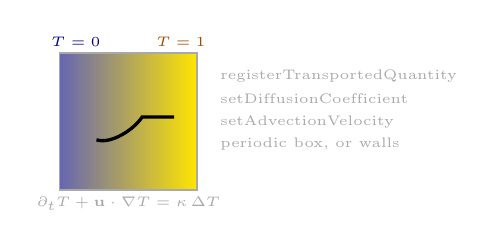
\begin{tikzpicture}[scale=0.58]
  \shade[left color=NavyBlue!60, right color=yellow!80!orange] (0,0) rectangle (3,3);
  \draw[DarkGray,thin] (0,0) rectangle (3,3);
  \draw[black,very thick] (0.8,1.1) .. controls (1.1,1.0) and (1.6,1.3) .. (1.8,1.6) -- (2.5,1.6);
  \node[font=\tiny,text=DarkGray] at (1.5,-0.3) {$\partial_t T + \mathbf{u}\cdot\nabla T = \kappa\,\Delta T$};
  \node[font=\tiny,text=NavyBlue] at (0.35,3.25) {$T = 0$};
  \node[font=\tiny,text=orange!60!black] at (2.65,3.25) {$T = 1$};
  \node[font=\tiny,text=DarkGray,anchor=west] at (3.3,2.5) {\code{registerTransportedQuantity}};
  \node[font=\tiny,text=DarkGray,anchor=west] at (3.3,2.0) {\code{setDiffusionCoefficient}};
  \node[font=\tiny,text=DarkGray,anchor=west] at (3.3,1.5) {\code{setAdvectionVelocity}};
  \node[font=\tiny,text=DarkGray,anchor=west] at (3.3,1.0) {periodic box, or walls};
\end{tikzpicture}}
\end{frame}

% 2
\begin{frame}{Learning goals}
\label{fr:goals}
\footnotesize By the end of this chapter you should be able to:
\begin{enumerate}
  \item write down what a passive scalar is, what the advection--diffusion equation says, and when diffusion matters against the grid's own smearing (the P\'eclet number and $\sqrt{\kappa t}$);
  \item add an advected and diffused quantity to any IBFE (or IB) program: the two headers, the solver object, the transported variable with its diffusion coefficient, initial condition, boundary conditions and advection velocity, and the one line that couples it to the fluid solver;
  \item choose between IBAMR's semi-implicit and predictor--corrector solvers for the scalar, write their input blocks, and know the one extra line the predictor--corrector needs with an Adams--Bashforth fluid solver;
  \item give the scalar initial and boundary conditions that agree with each other and with the box: periodic profiles in a periodic box, Robin conditions on walls, and the face numbering;
  \item explain what the course's linear profile did in a periodic box, measure it, and fix it;
  \item run IBFE/12, read its numbers, and look at $T$ with the moving plate in VisIt.
\end{enumerate}
\begin{punchbox}
\footnotesize One more equation, solved on the same grid by the same time integrator, with the velocity the IB method just computed. The structure never notices.
\end{punchbox}
\end{frame}

% 3
\begin{frame}{Where this chapter comes from}
\label{fr:sources}
\scriptsize
\begin{itemize}
  \item \al{``8-IBFE with Advection and Diffusion'' (July 2017; 14 slides):} the half-tethered plate of chapter 17 moving through ``a temperature (or concentration) gradient'' that ``begins as a linear function of $x$ with periodic boundary conditions''; four VisIt snapshots; the initial and boundary condition blocks; a review of Robin conditions and IBAMR's face numbering; the \code{main.C} and \code{input2d} additions, block by block.
  \item \al{``9-IBFE with Advection and Diffusion'' (2020; 18 slides; \code{IBFE\_Lecture\_9}):} the same deck pointing at the course example \code{9-IBFE\_TetherForceHalfPlate2D\_advdiff}, plus a last slide on rescaling the tether stiffness and the elastic modulus. The MATH 769 (2018) version is the same material.
  \item \al{The 2016 example zip} \code{Example\_IBFE\_TetherForceHalfPlate2D\_advdiff\_2016-11}: the course program and input the slides quote.
  \item \al{Example IBFE/12} (this series): the course program revised and run with IBAMR 0.16.0 and 0.19.0 (semi-implicit and predictor--corrector; the course's initial profile; walls; a larger $\kappa$), with the README's measured tables.
  \item \al{IBAMR 0.19.0:} \code{AdvDiffSemiImplicitHierarchyIntegrator}, \code{AdvDiffPredictorCorrectorHierarchyIntegrator} and their input keys; \code{examples/IB/explicit/ex7} (a point-method body with a dye) and \code{examples/adv\_diff/} (the scalar solvers on their own).
  \item \al{New here:} the equation and its scales; the solvers compared on the same run; the course input's solver line that was never read and the first-step error that follows; the jump the linear profile makes where the periodic box wraps, measured, and the periodic profile that replaces it; the figures from the shipped runs; the rescaling slide put in context.
\end{itemize}
\end{frame}

% 4
\begin{frame}{The equation, and its scales}
\label{fr:equation}
\footnotesize
\begin{columns}[T]
\column{0.52\textwidth}
A \emph{passive} scalar $T$ (a temperature, a concentration, a dye, oxygen) is carried by the velocity $\mathbf{u}$ the IB method computes and spreads by diffusion:
\[ \frac{\partial T}{\partial t} + \mathbf{u}\cdot\nabla T = \kappa\,\Delta T . \]
\begin{itemize}
  \item \al{Passive:} $T$ does not act back on the fluid or the body. One-way coupling: the fluid solver advances $\mathbf{u}$, then the scalar solver advances $T$ with that $\mathbf{u}$. (A scalar that changes the density or drives a force is a different, two-way problem.)
  \item \al{Advection} ($\mathbf{u}\cdot\nabla T$) moves the field with the fluid; \al{diffusion} ($\kappa\Delta T$) smooths it. Their ratio over a length $L$ at speed $U$ is the P\'eclet number $\mathrm{Pe} = UL/\kappa$.
  \item \al{The diffusion length} in a time $t$ is $\sqrt{\kappa t}$: how far a sharp edge spreads.
\end{itemize}
\column{0.46\textwidth}
In IBFE/12: $U = 0.5$ (the tether's speed), $L = 1$ (the plate), $\kappa = 10^{-6}$:
\begin{tabular}{@{}L{0.42\textwidth}L{0.5\textwidth}@{}}
\toprule
$\mathrm{Pe} = UL/\kappa$ & $5\times10^5$: advection dominates \\
$\sqrt{\kappa t}$ at $t = 4$ & $0.002$: less than one fine cell ($0.0156$) \\
with $\kappa = 10^{-3}$ & $0.063$: four fine cells \\
\bottomrule
\end{tabular}

\medskip
\begin{itemize}
  \item With $\kappa = 10^{-6}$ the physical diffusion is invisible on this grid; what smooths $T$ is the advection scheme itself (``numerical diffusion''), and the choice of scheme is what you see (slide \ref{fr:solvers2}).
  \item Water: heat $\kappa \approx 1.4\times10^{-3}$ cm$^2$/s, salt $\approx 1.5\times10^{-5}$, oxygen $\approx 2\times10^{-5}$: a dye in a 1 cm box at 0.5 cm/s is at $\mathrm{Pe} \sim 10^4$, and the same remark applies.
\end{itemize}
\end{columns}
\end{frame}

% 5
\begin{frame}{The example: the half-tethered plate stirs a field}
\label{fr:example}
\scriptsize
\begin{columns}[T]
\column{0.5\textwidth}
``This example includes a flexible plate that moves up then down that is tethered to target points on the one half of its length. A temperature (or concentration) gradient is considered that begins as a linear function of $x$ with periodic boundary conditions'' (2020, slide 2).
\begin{tabular}{@{}L{0.2\textwidth}L{0.74\textwidth}@{}}
\toprule
box & $2\times2$, periodic in $x$ and $y$; two levels, $32 \to 128$ cells, $\mathrm{DX} = 1/64$ \\
fluid & $\rho = 1$, $\mu = 0.01$ \\
plate & chapter 17's \code{IBFE\_Mesh2D\_128.mat}: $1\times0.0312$, $101$ nodes, $130$ triangles; neo-Hookean, $\mu_s = 10$ \\
tether & the right half ($s_0 > 0$), $\kappa_s = 10^6$; the target moves up at $0.5$ until $t = 1$, down until $t = 3$, then releases (IBFE/01, \code{MOTION = "HALF"}) \\
$T$ & $\kappa = 10^{-6}$; starts at $0$ on the plate's left end and $1$ on its right end \\
time & \code{DT = 1e-3}, $4000$ steps to $t = 4$, $41$ frames; about $90$ s on four cores \\
\bottomrule
\end{tabular}
\column{0.48\textwidth}
\centering
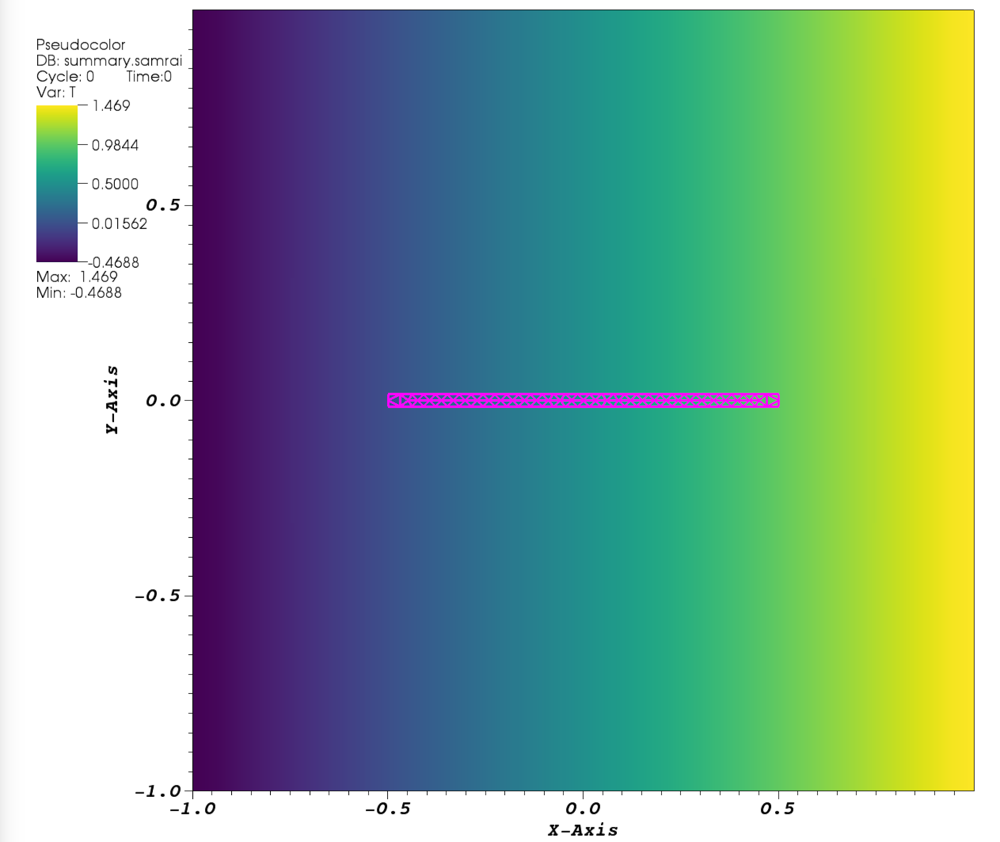
\includegraphics[width=0.47\textwidth]{ch24-2020-t0.png}\hfill
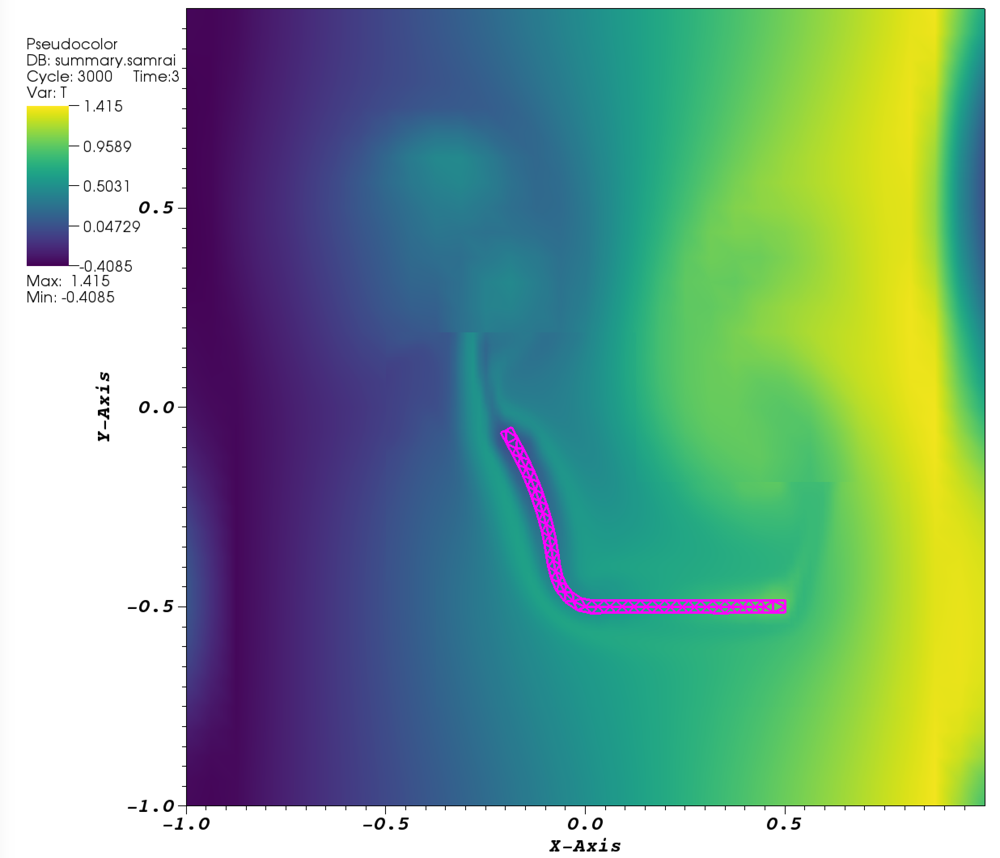
\includegraphics[width=0.47\textwidth]{ch24-2020-t3.png}\\
\scriptsize Two of the 2020 deck's four snapshots (slide 3): $T$ at $t = 0$ and $t = 3$ with the course's linear profile. Read the colour bar: $T$ runs from $-0.47$ to $1.47$, not from $0$ to $1$ (slide \ref{fr:jump}).
\end{columns}
\sourcecredit{Snapshots from the 2020 deck (Laura Miller, VisIt).}
\end{frame}

% 6
\begin{frame}[fragile]{The program (1): headers and the solver for $T$}
\label{fr:code1}
\footnotesize
\begin{lstlisting}[style=cpptiny]
// Headers for application-specific algorithm/data structure objects
#include <ibamr/AdvDiffPredictorCorrectorHierarchyIntegrator.h>
#include <ibamr/AdvDiffSemiImplicitHierarchyIntegrator.h>
...
// after the fluid solver, IBFEMethod and the IB time integrator exist (chapter 23, block 7):
Pointer<AdvDiffHierarchyIntegrator> adv_diff_integrator;
const string adv_diff_solver_type = input_db->getStringWithDefault("ADV_DIFF_SOLVER_TYPE", "SEMI_IMPLICIT");
if (adv_diff_solver_type == "PREDICTOR_CORRECTOR")
{
    Pointer<AdvectorExplicitPredictorPatchOps> predictor = new AdvectorExplicitPredictorPatchOps(
        "AdvectorExplicitPredictorPatchOps", app_initializer->getComponentDatabase("AdvectorExplicitPredictorPatchOps"));
    adv_diff_integrator = new AdvDiffPredictorCorrectorHierarchyIntegrator(
        "AdvDiffPredictorCorrectorHierarchyIntegrator",
        app_initializer->getComponentDatabase("AdvDiffPredictorCorrectorHierarchyIntegrator"), predictor);
}
else if (adv_diff_solver_type == "SEMI_IMPLICIT")
{
    adv_diff_integrator = new AdvDiffSemiImplicitHierarchyIntegrator(
        "AdvDiffSemiImplicitHierarchyIntegrator", app_initializer->getComponentDatabase("AdvDiffSemiImplicitHierarchyIntegrator"));
}
else
{
    TBOX_ERROR("Unsupported ADV_DIFF_SOLVER_TYPE: " << adv_diff_solver_type << "\n" << "Valid options are: PREDICTOR_CORRECTOR, SEMI_IMPLICIT");
}
pout << "Advection-diffusion solver: " << adv_diff_solver_type << "\n";
navier_stokes_integrator->registerAdvDiffHierarchyIntegrator(adv_diff_integrator);
\end{lstlisting}
\end{frame}

% 6a
\begin{frame}{The program (1a): what the solver block does}
\label{fr:code1a}
\footnotesize
\begin{itemize}
  \item ``After you create the major algorithm and data objects that comprise the application (e.g.\ setting the solver\_type, IBFE method, etc.) add the following for the adv diff solver'' (2020, slide 13). The last line is the coupling: the fluid integrator now owns a scalar integrator and advances it inside every one of its own steps, with the velocity it has just computed.
  \item \code{AdvDiffHierarchyIntegrator} is the base class of both solvers, as \code{INSHierarchyIntegrator} is of the two fluid solvers (chapter 23).
\end{itemize}
\end{frame}

% 6b
\begin{frame}[fragile]{The program (1b): the solver line the course input never reached}
\label{fr:code1b}
\footnotesize
The 2017 and 2020 slides read the choice from the \code{Main} block:
\begin{lstlisting}[style=cpptiny]
Pointer<Database> main_db = app_initializer->getComponentDatabase("Main");
const string adv_diff_solver_type = main_db->getStringWithDefault("adv_diff_solver_type", "PREDICTOR_CORRECTOR");
\end{lstlisting}
while the input defined \code{ADV\_DIFF\_SOLVER\_TYPE = "SEMI\_IMPLICIT"} at the top (slide 14) and never put \code{adv\_diff\_solver\_type = ADV\_DIFF\_SOLVER\_TYPE} into \code{Main}: the slides did not show that line.
\begin{itemize}
  \item So a program and input copied from the slides use the \emph{default}, \code{PREDICTOR\_CORRECTOR}, whatever the top of the input says, and stop at the first step (slide \ref{fr:cycles}). Tested with the course program and IBAMR 0.19.0.
  \item IBFE/12 reads \code{ADV\_DIFF\_SOLVER\_TYPE} from the top level directly, defaults to \code{SEMI\_IMPLICIT}, and prints its choice at the start of the run (``\code{Advection-diffusion solver: SEMI\_IMPLICIT}''), so the log says which solver ran.
  \item Chapter 23's rule again: a key is read only where the program looks for it, and the log's \code{// input used} marks tell you.
\end{itemize}
\end{frame}

% 7
\begin{frame}[fragile]{The program (2): the transported quantity}
\label{fr:code2}
\footnotesize
\begin{lstlisting}[style=cpptiny]
const bool periodic_domain = grid_geometry->getPeriodicShift().min() > 0;
// Setup the advected and diffused quantity.
Pointer<CellVariable<NDIM, double> > T_var = new CellVariable<NDIM, double>("T");
adv_diff_integrator->registerTransportedQuantity(T_var);
adv_diff_integrator->setDiffusionCoefficient(T_var, input_db->getDouble("KAPPA"));
Pointer<CartGridFunction> T_init = new muParserCartGridFunction(
    "T_init", app_initializer->getComponentDatabase("TemperatureInitialConditions"), grid_geometry);
adv_diff_integrator->setInitialConditions(T_var, T_init);
std::unique_ptr<RobinBcCoefStrategy<NDIM> > T_bc_coef;
if (!periodic_domain)
{
    T_bc_coef = std::make_unique<muParserRobinBcCoefs>(
        "T_bc_coef", app_initializer->getComponentDatabase("TemperatureBcCoefs"), grid_geometry);
    adv_diff_integrator->setPhysicalBcCoef(T_var, T_bc_coef.get());
}
adv_diff_integrator->setAdvectionVelocity(T_var, navier_stokes_integrator->getAdvectionVelocityVariable());
\end{lstlisting}
\begin{itemize}
  \item ``Before you Configure the IBFE solver in main.C, add these lines (note they go after the pointers for load balancers and gridding algorithms)'' (2020, slide 12): block 8 of chapter 23's map, before block 9.
  \item Five calls, in this order: the variable (a cell-centred field named \code{T}, which is the name VisIt will show), its diffusion coefficient, its initial condition (a muParser block, like the velocity's), its boundary conditions (only if the box is not periodic; a periodic box overrides them), and the velocity that carries it, which is the fluid solver's own advection velocity.
  \item The 2020 code held the boundary object in a raw pointer set to \code{NULL} and never deleted it; IBFE/12 uses a \code{unique\_ptr}. A second scalar is five more lines with another name.
\end{itemize}
\end{frame}

% 8
\begin{frame}[fragile]{The input (1): the keys and the two solver blocks}
\label{fr:input}
\footnotesize
\begin{columns}[T]
\column{0.5\textwidth}
\begin{lstlisting}[style=inputtiny]
KAPPA = 1.0e-6                   // temperature diffusion coefficient
...
ADV_DIFF_SOLVER_TYPE        = "SEMI_IMPLICIT"   // or PREDICTOR_CORRECTOR
ADV_DIFF_NUM_CYCLES         = 2                 // fixed-point cycles
ADV_DIFF_CONVECTIVE_TS_TYPE = "MIDPOINT_RULE"   // time stepping
ADV_DIFF_CONVECTIVE_OP_TYPE = "PPM"             // spatial scheme
ADV_DIFF_CONVECTIVE_FORM    = "ADVECTIVE"       // or CONSERVATIVE
DT_MAX                      = 0.1               // its own step limit
...
AdvDiffSemiImplicitHierarchyIntegrator {
   start_time                    = START_TIME
   end_time                      = END_TIME
   grow_dt                       = GROW_DT
   num_cycles                    = ADV_DIFF_NUM_CYCLES
   convective_time_stepping_type = ADV_DIFF_CONVECTIVE_TS_TYPE
   convective_op_type            = ADV_DIFF_CONVECTIVE_OP_TYPE
   convective_difference_form    = ADV_DIFF_CONVECTIVE_FORM
   cfl                           = CFL_MAX
   dt_max                        = DT_MAX
   tag_buffer                    = TAG_BUFFER
   enable_logging                = ENABLE_LOGGING
}
\end{lstlisting}
\column{0.48\textwidth}
\begin{lstlisting}[style=inputtiny]
AdvDiffPredictorCorrectorHierarchyIntegrator {
   start_time                 = START_TIME
   end_time                   = END_TIME
   grow_dt                    = GROW_DT
   convective_difference_form = ADV_DIFF_CONVECTIVE_FORM
   cfl                        = CFL_MAX
   dt_max                     = DT_MAX
   tag_buffer                 = TAG_BUFFER
   enable_logging             = ENABLE_LOGGING
   AdvDiffPredictorCorrectorHyperbolicPatchOps {
      compute_init_velocity  = TRUE
      compute_half_velocity  = TRUE
      compute_final_velocity = FALSE
      extrap_type = "LINEAR"
   }
   HyperbolicLevelIntegrator {
      cfl                      = CFL_MAX
      cfl_init                 = CFL_MAX
      lag_dt_computation       = TRUE
      use_ghosts_to_compute_dt = FALSE
   }
}
AdvectorExplicitPredictorPatchOps {
   limiter_type = "MC_LIMITED"
}
\end{lstlisting}
\vspace{-4pt}\tiny ``Add these to the bottom of the list of solver parameters \ldots Add a diffusion coefficient to the physical parameters \ldots Add settings for advection diffusion solver'' (2020, slides 14--17). Both blocks are in the input, so the switch works; only the chosen one is read.
\end{columns}
\end{frame}

% 8b
\begin{frame}{The input (2): what the keys mean, and their aliases}
\label{fr:keys}
\scriptsize
\setlength{\tabcolsep}{3pt}
\begin{tabular}{@{}L{0.26\textwidth}L{0.66\textwidth}@{}}
\toprule
key & meaning (and the spellings \code{getFromInput} accepts) \\
\midrule
\code{num\_cycles} & fixed-point iterations per step of the semi-implicit solver; $2$ here, the fluid solver's own number \\
\code{convective\_time\_}\newline\code{stepping\_type} & how the advection term is stepped: \code{MIDPOINT\_RULE}, \code{ADAMS\_BASHFORTH}, \code{FORWARD\_EULER}, \code{TRAPEZOIDAL\_RULE}; also \code{convective\_timestepping\_type}, \code{default\_convective\_time\_stepping\_type} \\
\code{init\_convective\_}\newline\code{time\_stepping\_type} & the same for the first step, when there is no previous step to extrapolate from (slide \ref{fr:cycles}) \\
\code{convective\_op\_type} & the spatial scheme: \code{PPM} (piecewise parabolic), \code{CENTERED}, \code{CUI}, \code{WAVE\_PROP}; also \code{convective\_operator\_type} \\
\code{convective\_difference\_form} & \code{ADVECTIVE} ($\mathbf{u}\cdot\nabla T$) or \code{CONSERVATIVE} ($\nabla\cdot(\mathbf{u}T)$); also \code{\_type} \\
\code{diffusion\_time\_}\newline\code{stepping\_type} & how $\kappa\Delta T$ is stepped (implicit; the trapezoidal rule by default) \\
\code{cfl}, \code{cfl\_max}, \code{CFL}, \code{CFL\_max} & the scalar solver's own CFL limit on its step \\
\code{dt\_max} & its own step limit, which the fluid's step then also bounds: \code{DT\_MAX = 0.1} does nothing here against \code{DT = 1e-3} \\
\code{limiter\_type} (predictor) & the slope limiter of the Godunov predictor: \code{MC\_LIMITED}, \code{MINMOD\_LIMITED}, \code{SUPERBEE\_LIMITED}, \code{NONE} \\
\bottomrule
\end{tabular}

\medskip
\begin{itemize}
  \item The scalar solver's step is the fluid's step: \code{registerAdvDiffHierarchyIntegrator} makes the fluid integrator call it once per fluid step (or per cycle). Its own \code{dt\_max} and \code{cfl} only matter if they are \emph{smaller} than the fluid's.
  \item \code{tag\_buffer}, \code{start\_time}, \code{end\_time}, \code{grow\_dt} repeat the fluid's values; they must not disagree.
\end{itemize}
\end{frame}

% 9
\begin{frame}{The two solvers}
\label{fr:solvers}
\footnotesize
\begin{tabular}{@{}L{0.2\textwidth}L{0.36\textwidth}L{0.36\textwidth}@{}}
\toprule
& \code{SEMI\_IMPLICIT} & \code{PREDICTOR\_CORRECTOR} \\
\midrule
advection & explicit, the fluid solver's own scheme (PPM with the midpoint rule here), with \code{num\_cycles} fixed-point sweeps & an explicit Godunov predictor (the class \code{AdvectorExplicit}\newline\code{PredictorPatchOps}): upwind with a slope limiter, the half-step velocity, corner transport \\
diffusion & implicit (trapezoidal rule) & implicit \\
overshoot & can overshoot a little where the field folds ($1.008$ and $-0.003$ on a field between $0$ and $1$) & none: the limiter keeps $T$ within its starting range; the extremes wear down instead ($0.9998 \to 0.9965$ by $t = 4$) \\
first step & no requirement & one cycle only: the fluid solver's first step must be single-cycle too (slide \ref{fr:cycles}) \\
when & the default; the same scheme as the fluid, one set of settings & a bounded scalar (a concentration that must stay in $[0, 1]$), or a sharp front \\
\bottomrule
\end{tabular}

\medskip
\begin{itemize}
  \item Both solve $\partial_t T + \mathbf{u}\cdot\nabla T = \kappa\Delta T$ on the same adaptive grid with the velocity the fluid solver provides; the difference is the advection scheme, and at $\mathrm{Pe} = 5\times10^5$ that difference is what you see (slide \ref{fr:solvers2}).
  \item \code{examples/adv\_diff/} in IBAMR runs the two solvers without any body: \code{ex0}--\code{ex8}, with analytic solutions to compare against, are where to go when a scalar result looks wrong.
\end{itemize}
\end{frame}

% 9b
\begin{frame}[fragile]{The predictor--corrector's one extra line}
\label{fr:cycles}
\scriptsize
With \code{ADV\_DIFF\_SOLVER\_TYPE = "PREDICTOR\_CORRECTOR"} and nothing else changed, the run stops at the first step:
\begin{lstlisting}[style=tiny]
INSStaggeredHierarchyIntegrator::preprocessIntegrateHierarchy():
  attempting to perform 2 cycles of fixed point iteration.
  number of cycles required by coupled advection-diffusion solver = 1.
  current implementation requires either that both solvers use the same number of cycles,
  or that the Navier-Stokes solver use only a single cycle.
\end{lstlisting}
\begin{itemize}
  \item The fluid solver steps its convective term with Adams--Bashforth, which has no previous step at $t = 0$ and so takes \emph{two} cycles for the first step; the predictor--corrector scalar solver can take only one. The two must agree.
  \item The fix is one line in the \code{INSStaggeredHierarchyIntegrator} block, shipped commented out in IBFE/12's input:
\end{itemize}
\begin{lstlisting}[style=inputtiny]
INSStaggeredHierarchyIntegrator {
   ...
   // init_convective_time_stepping_type = "FORWARD_EULER"   // remove the // for PREDICTOR_CORRECTOR
}
\end{lstlisting}
\begin{itemize}
  \item The first fluid step then uses forward Euler for its convective term, a single cycle, and the rest of the run is unchanged (Adams--Bashforth from the second step on).
  \item This is the error the course's slides would have produced on current IBAMR, through the unread key of slide \ref{fr:code1b}: the course program defaulted to the predictor--corrector, and the input had no single-cycle first step.
\end{itemize}
\end{frame}

% 10
\begin{frame}[fragile]{Initial and boundary conditions for $T$}
\label{fr:icbc}
\footnotesize
\begin{columns}[T]
\column{0.5\textwidth}
\begin{lstlisting}[style=inputtiny]
TemperatureInitialConditions {
   // the course's profile, 0.5 + x: see the next slides
   // function = "0.5+X_0"
   // two of the course's other trials (they jump where the box wraps in y)
   // function = "0.5*(tanh(80.0*(-X_1-0.15))+1)"
   // function = "(0.5*(tanh(80.0*(-X_1-0.15))+1))*(0.5*(tanh(80.0*(X_0+0.115))+1))*(0.5*(tanh(80.0*(-X_0+0.115))+1))"
   L = L
   function = "0.5 + 0.5*sin(2*PI*X_0/L)"
}
TemperatureBcCoefs {   // read only on sides that are not periodic
   L = L
   acoef_function_0 = "1.0"   ...   acoef_function_3 = "1.0"
   bcoef_function_0 = "0.0"   ...   bcoef_function_3 = "0.0"
   gcoef_function_0 = "0.5 + 0.5*sin(2*PI*X_0/L)"   ...   gcoef_function_3 = "0.5 + 0.5*sin(2*PI*X_0/L)"
}
\end{lstlisting}
\scriptsize ``The boundary conditions are set up the same way as the velocity boundary conditions (e.g.\ periodic or Robin boundary conditions). In this example, the boundary conditions are periodic (overrides Robin) and the initial concentration is a linear function of $x$'' (2020, slide 4).
\column{0.48\textwidth}
\begin{itemize}
  \item \al{The initial condition} is any muParser expression of \code{X\_0}, \code{X\_1} (and \code{X\_2}) and the block's own constants; chapter 7's rules for the velocity's blocks apply, including that a block sees only its own constants (\code{L = L} copies it in).
  \item \al{Periodic overrides Robin:} on a periodic side the block is never read; the two sides are the same place.
\end{itemize}
\end{columns}
\end{frame}

% 10a
\begin{frame}{Initial and boundary conditions (2): Robin conditions}
\label{fr:robin}
\footnotesize
\begin{itemize}
  \item \al{The boundary condition} is Robin on each face: $a\,T + b\,\partial T/\partial n = g$. ``Robin boundary conditions are a weighted combination of Dirichlet boundary conditions and Neumann boundary conditions'' (2020, slide 8). $a = 1$, $b = 0$: $T = g$ on the face (a wall held at a temperature); $a = 0$, $b = 1$: $\partial T/\partial n = g$ (an insulated wall for $g = 0$; a prescribed flux otherwise); both non-zero: a wall that exchanges heat with its surroundings at a rate set by $b/a$.
  \item \al{The sign} of the normal: ``In one dimension, if $\Omega = [0, 1]$, the Robin boundary condition becomes $a u(0) - b u'(0) = g(0)$, $a u(1) + b u'(1) = g(1)$. Notice the change of sign \ldots because the normal at $x = 0$ points in the negative direction'' (slide 9). IBAMR's $\partial/\partial n$ is the outward normal derivative on every face, so the input never carries that sign: $b = 1$, $g = 0$ is ``no flux'' on any face.
  \item The velocity's conditions (chapter 7) are the same objects with the same keys, one block per component; a scalar needs one block.
  \item \al{Initial and boundary values must agree} where they meet: a wall held at $T = g$ next to an initial field with a different value there starts the run with a jump at the wall, the same trouble as slide \ref{fr:jump} in another place.
\end{itemize}
\end{frame}


% 10b
\begin{frame}{The faces, numbered}
\label{fr:faces}
\footnotesize
\begin{columns}[T]
\column{0.42\textwidth}
\begin{center}
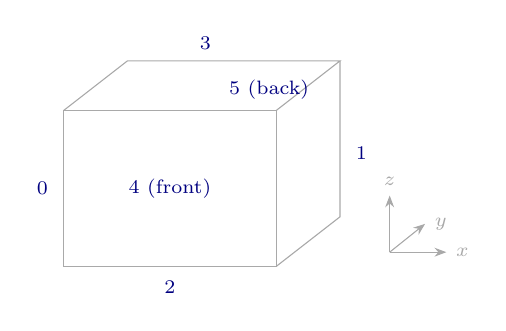
\begin{tikzpicture}[scale=0.9, every node/.style={font=\scriptsize}]
  \draw[DarkGray] (0,0) rectangle (3,2.2);
  \draw[DarkGray] (0,2.2) -- (0.9,2.9) -- (3.9,2.9) -- (3,2.2);
  \draw[DarkGray] (3,0) -- (3.9,0.7) -- (3.9,2.9);
  \node[text=NavyBlue] at (-0.3,1.1) {0};
  \node[text=NavyBlue] at (4.2,1.6) {1};
  \node[text=NavyBlue] at (1.5,-0.3) {2};
  \node[text=NavyBlue] at (2.0,3.15) {3};
  \node[text=NavyBlue] at (1.5,1.1) {4 (front)};
  \node[text=NavyBlue] at (2.9,2.5) {5 (back)};
  \draw[-{Stealth[length=1.5mm]},DarkGray] (4.6,0.2) -- (5.4,0.2) node[right] {$x$};
  \draw[-{Stealth[length=1.5mm]},DarkGray] (4.6,0.2) -- (4.6,1.0) node[above] {$z$};
  \draw[-{Stealth[length=1.5mm]},DarkGray] (4.6,0.2) -- (5.1,0.6) node[right] {$y$};
\end{tikzpicture}
\end{center}
\scriptsize Redrawn from the 2020 deck's slide 10 (a box of unknown origin with the faces numbered).
\column{0.56\textwidth}
``IBAMR boundary numbering. Look in the input2D/3D files. 2D: xleft = 0, xright = 1, ybottom = 2, ytop = 3. 3D: add zbottom = 4, ztop = 5'' (2020, slide 10).
\begin{itemize}
  \item The rule: face $2d$ is the low side of direction $d$ and face $2d + 1$ the high side; $d = 0, 1, 2$ for $x, y, z$. The same numbering serves \code{VelocityBcCoefs\_d}, \code{TemperatureBcCoefs}, the sponge layer of chapter 23 and the output of the \code{SpongeLayerForceFunction} keys.
  \item The \code{\_d} in \code{VelocityBcCoefs\_d} is the velocity \emph{component}; the \code{\_0} to \code{\_5} in \code{gcoef\_function\_0} is the \emph{face}. A scalar has one block with six faces; a velocity has three blocks with six faces each.
  \item In the chapter 22 tank the $x$-velocity was set on all six faces (\code{gcoef\_function\_0} to \code{\_5} of \code{VelocityBcCoefs\_0}); here, with periodicity on, no face is read at all.
\end{itemize}
\end{columns}
\end{frame}

% 11
\begin{frame}{The jump the linear profile hid}
\label{fr:jump}
\scriptsize
\begin{columns}[T]
\column{0.5\textwidth}
\begin{itemize}
  \item ``The temperature is a linear function of $x$ which has an initial range of $-0.5$ to $1.5$'' (2020, slide 5): $T = 0.5 + x$ on $-1 < x < 1$ gives $0$ at the plate's left end and $1$ at its right end, which was the intent.
  \item But the box is periodic: $x = 1$ touches $x = -1$. The profile is $1.5$ on one side of that seam and $-0.5$ on the other, a \al{jump of $2$} at the edge of the box, carried into the fluid as soon as anything moves there. The colour bar on the course's snapshots ($-0.47$ to $1.47$) is this jump.
  \item \al{Measured} (the course program, IBAMR 0.19.0): in the coarse cell next to the right side of the box at mid-height ($x = 0.97$, $y = 0.03$), $T$ starts at $1.47$ and falls to $-0.16$ by $t = 4$: fluid that leaves through the left side, where $T \approx -0.5$, comes back in through the right. The average of $T$ over the box, which should stay $0.5$, falls to $0.495$.
\end{itemize}
\column{0.48\textwidth}
\centering
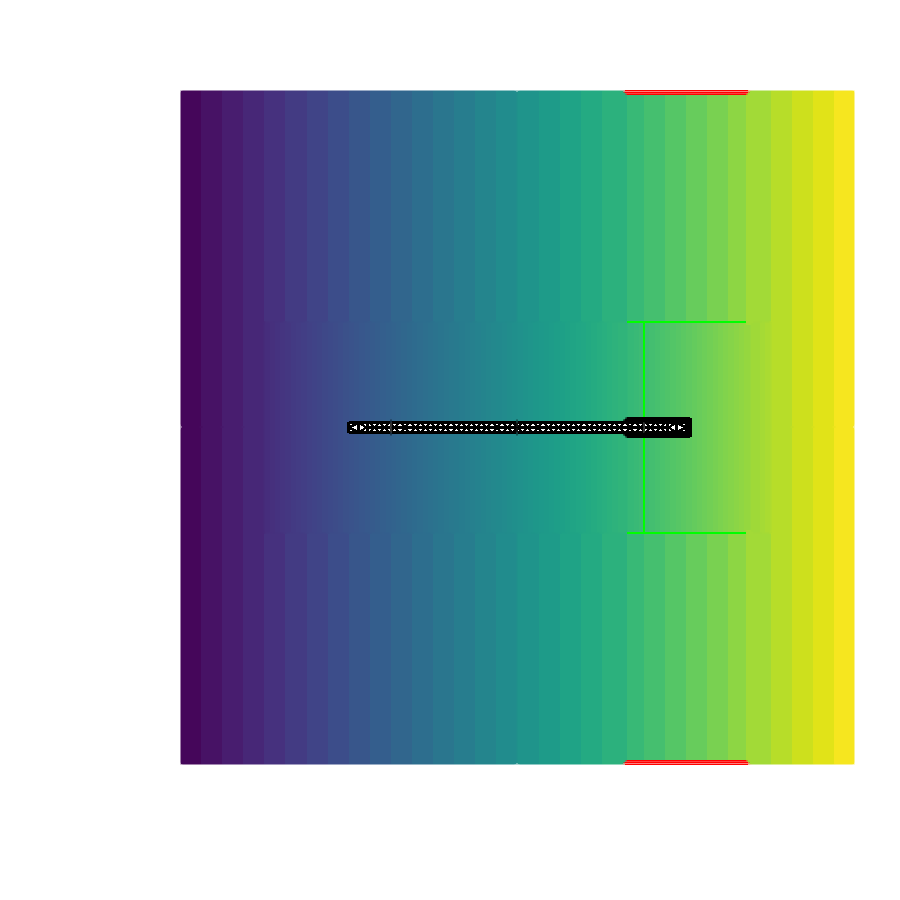
\includegraphics[width=0.48\textwidth]{ch24-course-ic-t0.png}\hfill
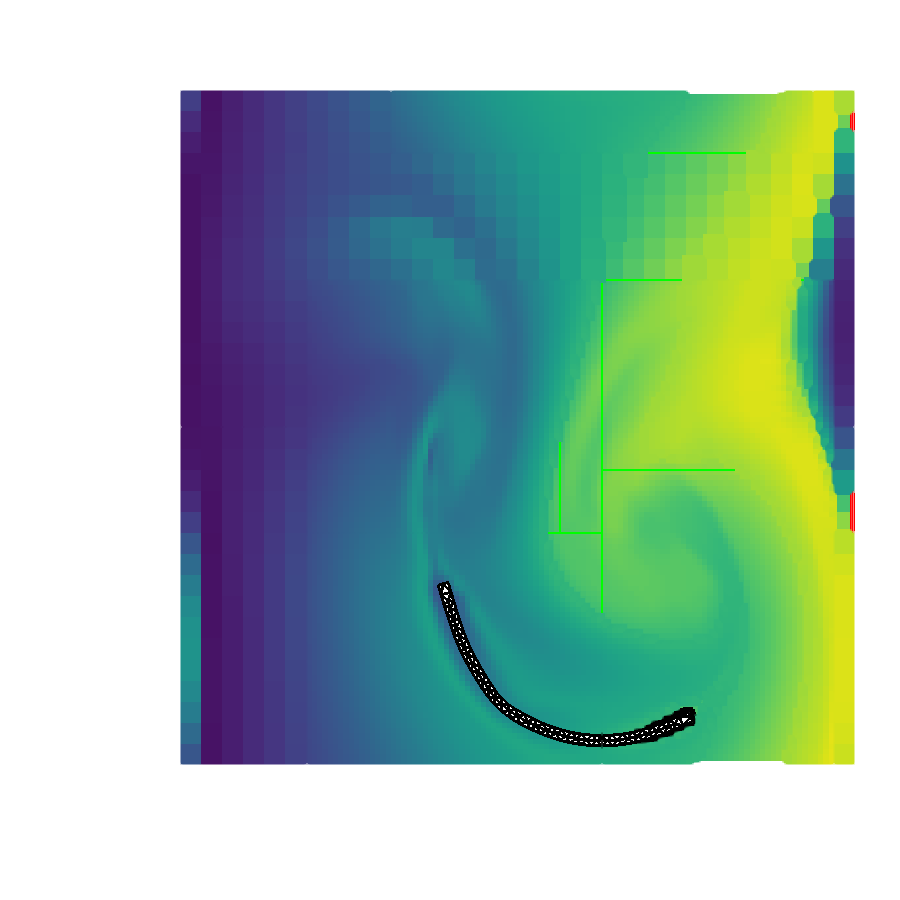
\includegraphics[width=0.48\textwidth]{ch24-course-ic-t4.png}\\
\scriptsize The course's $T = 0.5 + x$ at $t = 0$ and $t = 4$ (colour from $-0.5$ to $1.5$): the seam at the left and right edges is where $1.5$ meets $-0.5$.
\end{columns}
\begin{punchbox}
\footnotesize In a periodic box the initial field must be periodic too: same value, and ideally the same slope, on the two sides of every periodic direction. The same holds for the velocity and for any forcing.
\end{punchbox}
\end{frame}

% 11b
\begin{frame}{The jump (2): two fixes}
\label{fr:fixes}
\footnotesize
\begin{columns}[T]
\column{0.5\textwidth}
\al{Keep the box periodic, make the profile periodic} (IBFE/12):
\[ T = \tfrac12 + \tfrac12\sin\!\left(\frac{2\pi x}{L}\right), \qquad L = 2, \]
which is $0$, $\tfrac12$ and $1$ at $x = -\tfrac12$, $0$ and $\tfrac12$, the three values the course formula had on the plate, and $\tfrac12$ with the same slope at both edges of the box. $T$ stays between $0$ and $1$ and its average stays $\tfrac12$ (slide \ref{fr:see}).

\medskip
\al{Or put walls round the box} and hold $T$ on them: \code{periodic\_dimension = 0,0}, no-slip velocity on the four faces, and \code{TemperatureBcCoefs} with $a = 1$, $b = 0$, $g$ = the initial profile, so that the initial and boundary values agree on the walls. Any profile then works, the linear one included.
\column{0.48\textwidth}
\centering
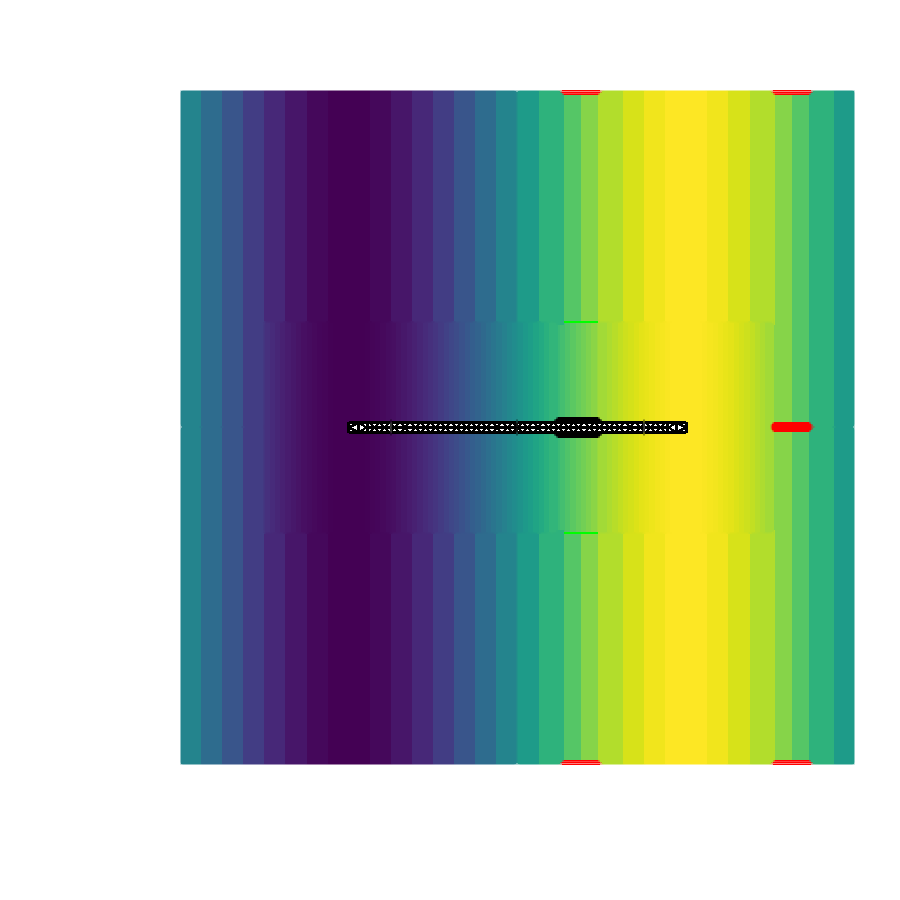
\includegraphics[width=0.55\textwidth]{ch24-T-t0.png}\\
\scriptsize IBFE/12's periodic profile at $t = 0$ (colour from $0$ to $1$).
\begin{itemize}
  \item With walls the plate moves differently (by up to $0.15$ at $t = 4$: the walls are only one plate-length away), and $T$ stays within $-0.033$ and $1.015$ (slide \ref{fr:variants}).
  \item The course's two other trials, \code{tanh} profiles in $y$ (kept as comments in the input), jump where the box wraps in $y$; the same rule, the other direction.
\end{itemize}
\end{columns}
\end{frame}

% 12
\begin{frame}{What you should see (1): the plate folds the field}
\label{fr:see}
\begin{columns}[T]
\column{0.2\textwidth}\centering 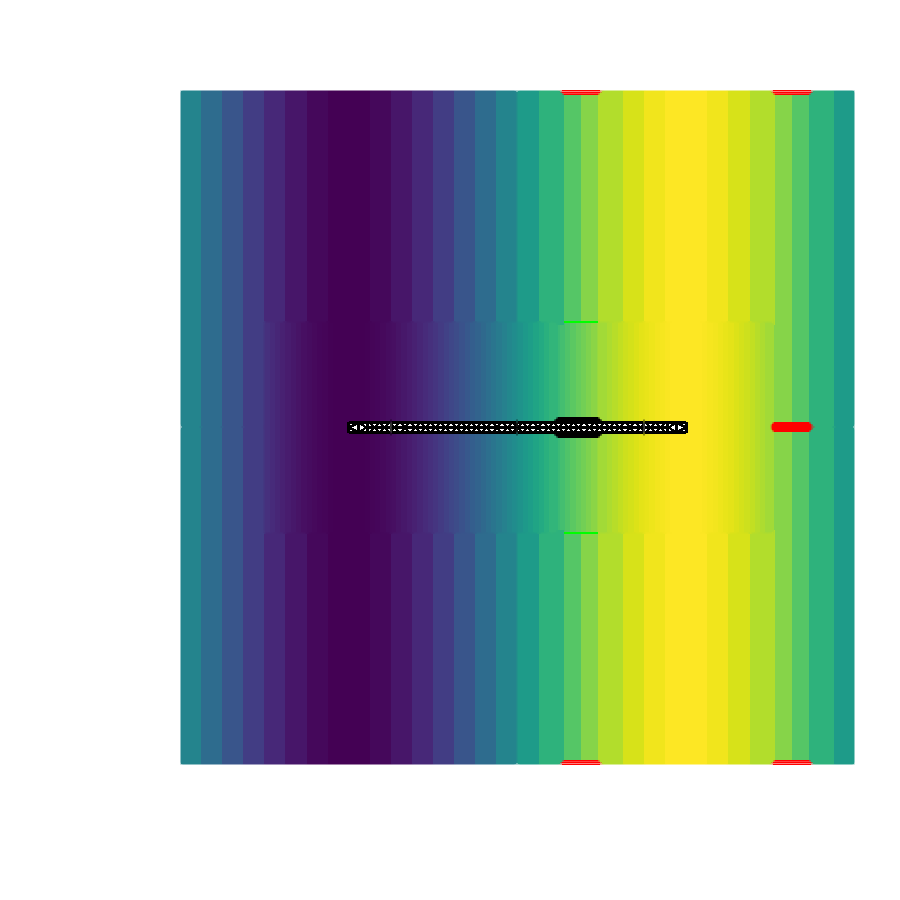
\includegraphics[width=0.85\textwidth]{ch24-T-t0.png}\\ \tiny $t = 0$
\column{0.2\textwidth}\centering 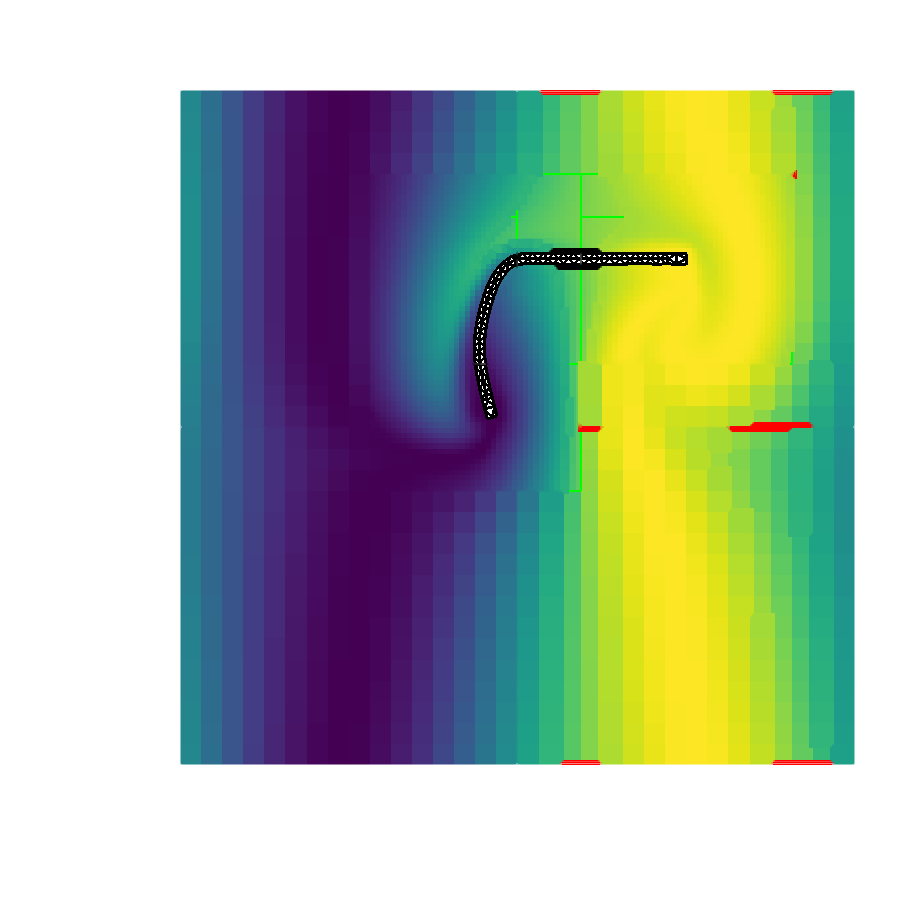
\includegraphics[width=0.85\textwidth]{ch24-T-t1.png}\\ \tiny $t = 1$: the tethered half has risen $0.5$
\column{0.2\textwidth}\centering 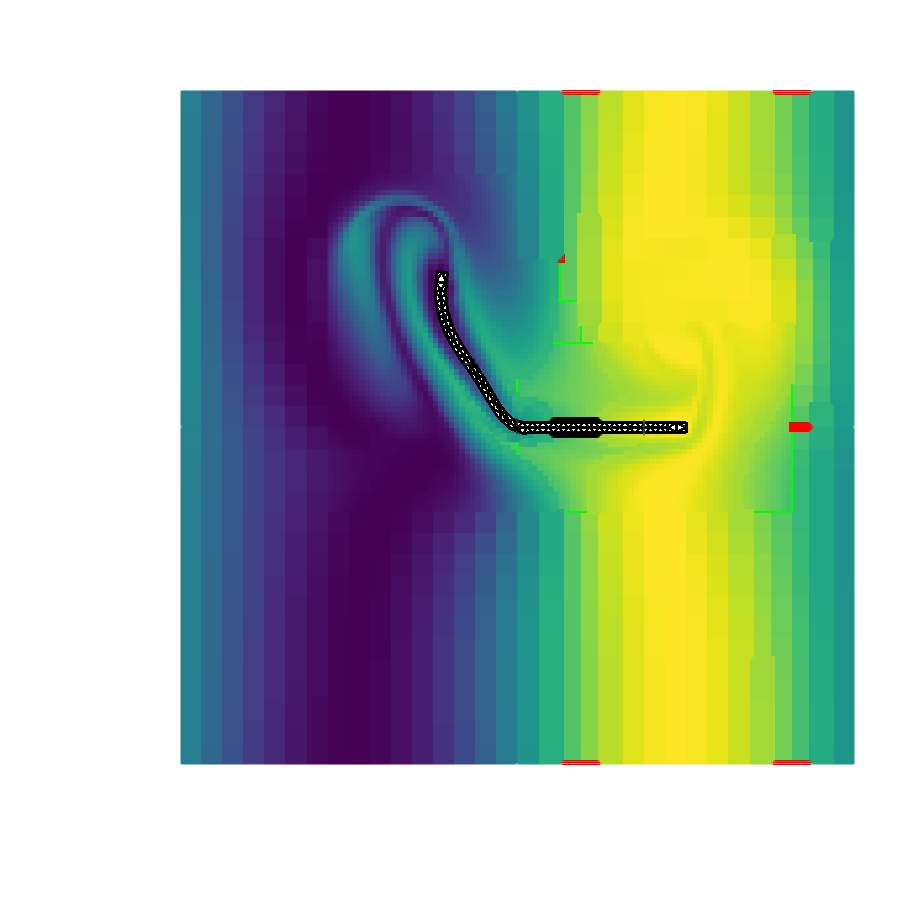
\includegraphics[width=0.85\textwidth]{ch24-T-t2.png}\\ \tiny $t = 2$: on the way down
\column{0.2\textwidth}\centering 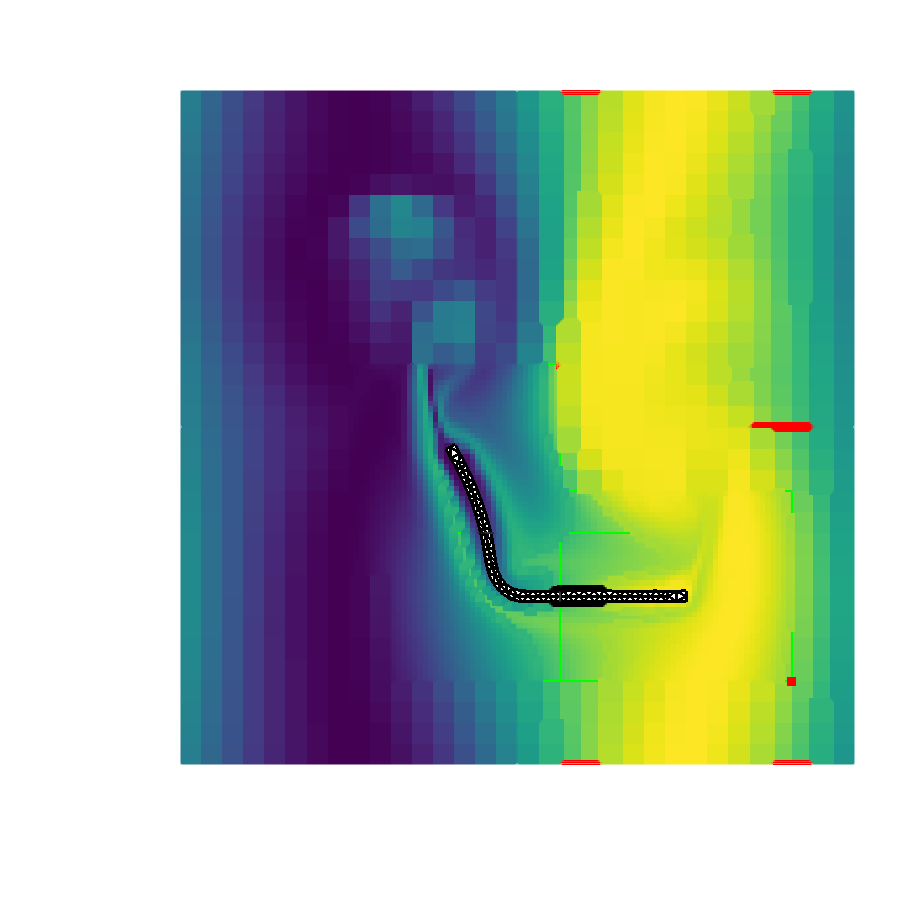
\includegraphics[width=0.85\textwidth]{ch24-T-t3.png}\\ \tiny $t = 3$: released
\column{0.2\textwidth}\centering 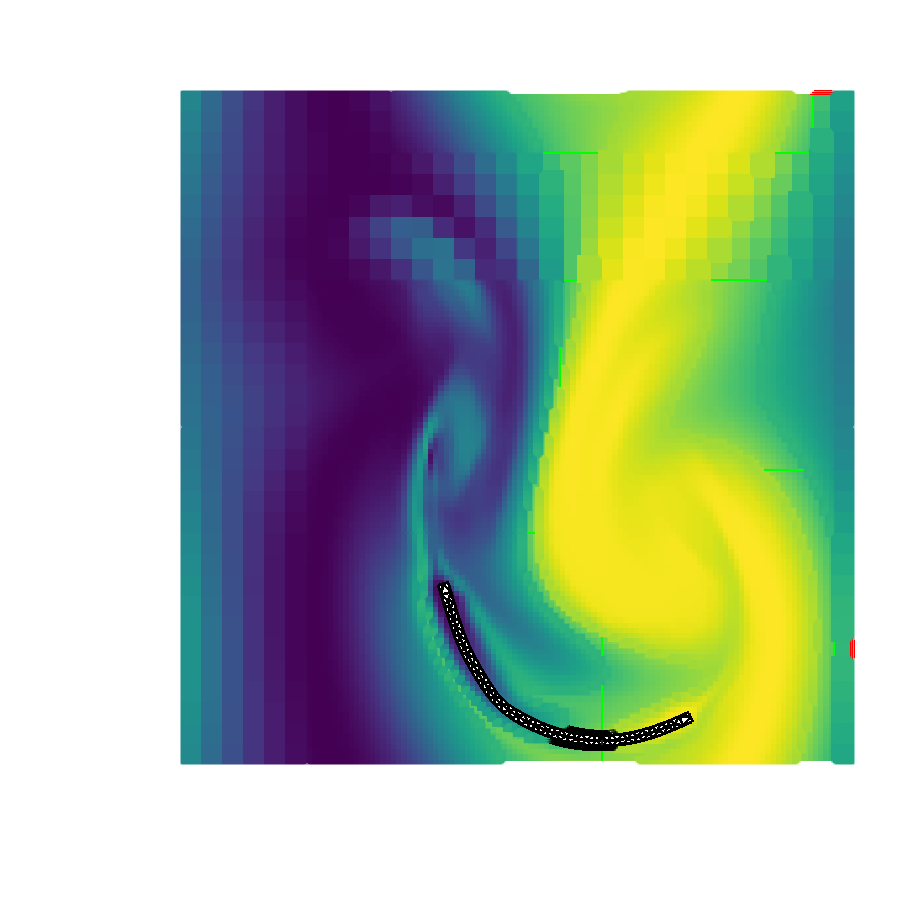
\includegraphics[width=0.85\textwidth]{ch24-T-t4.png}\\ \tiny $t = 4$: coasting
\end{columns}
\scriptsize
\begin{itemize}
  \item $T$ from $0$ (dark) to $1$ (yellow); the plate in black, displaced by \code{dX}. The free half trails the tethered half (chapter 17), and the field is folded by the flow the plate drives: the stripes are the initial profile, stretched and wrapped.
  \item The plate's motion is IBFE/01's to $2\times10^{-8}$: the scalar changes nothing on the fluid or the body.
  \item Each place is counted once, on the finest grid that covers it (chapter 29's queries):
\end{itemize}
\begin{center}\scriptsize
\begin{tabular}{@{}lllll@{}}
\toprule
$t$ & $0$ & $1$ & $2$ & $4$ \\
\midrule
smallest $T$ & $0.0002$ & $-0.0031$ & $-0.0012$ & $-0.0006$ \\
largest $T$ & $0.9998$ & $1.0003$ & $1.0000$ & $1.0053$ \\
average $T$ & $0.50000$ & $0.49995$ & $0.50001$ & $0.49992$ \\
\bottomrule
\end{tabular}
\end{center}
\sourcecredit{IBFE/12, IBAMR 0.19.0 (\code{/root/work/0.19.0/ibfe12\_final}); \code{wsl/final/visit\_ch24.sh}. 0.16.0 gives the same numbers.}
\end{frame}

% 13
\begin{frame}{What you should see (2): the variants at $t = 4$}
\label{fr:variants}
\begin{columns}[T]
\column{0.25\textwidth}\centering 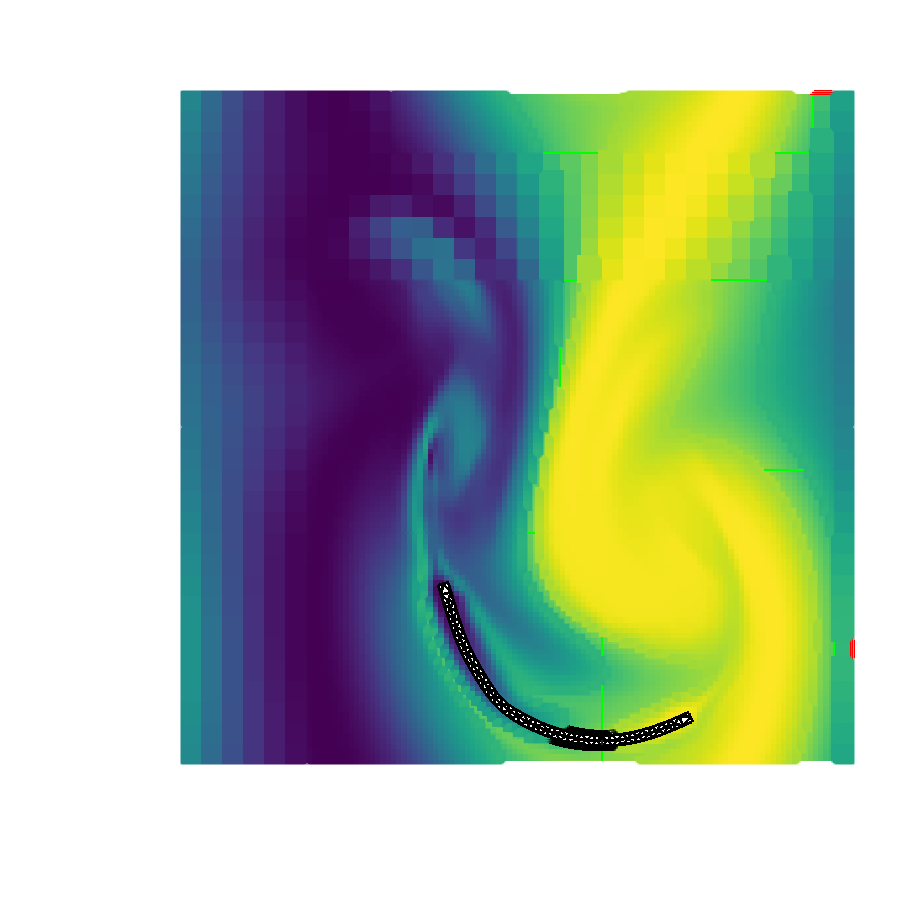
\includegraphics[width=\textwidth]{ch24-T-t4.png}\\ \scriptsize semi-implicit, $\kappa = 10^{-6}$
\column{0.25\textwidth}\centering 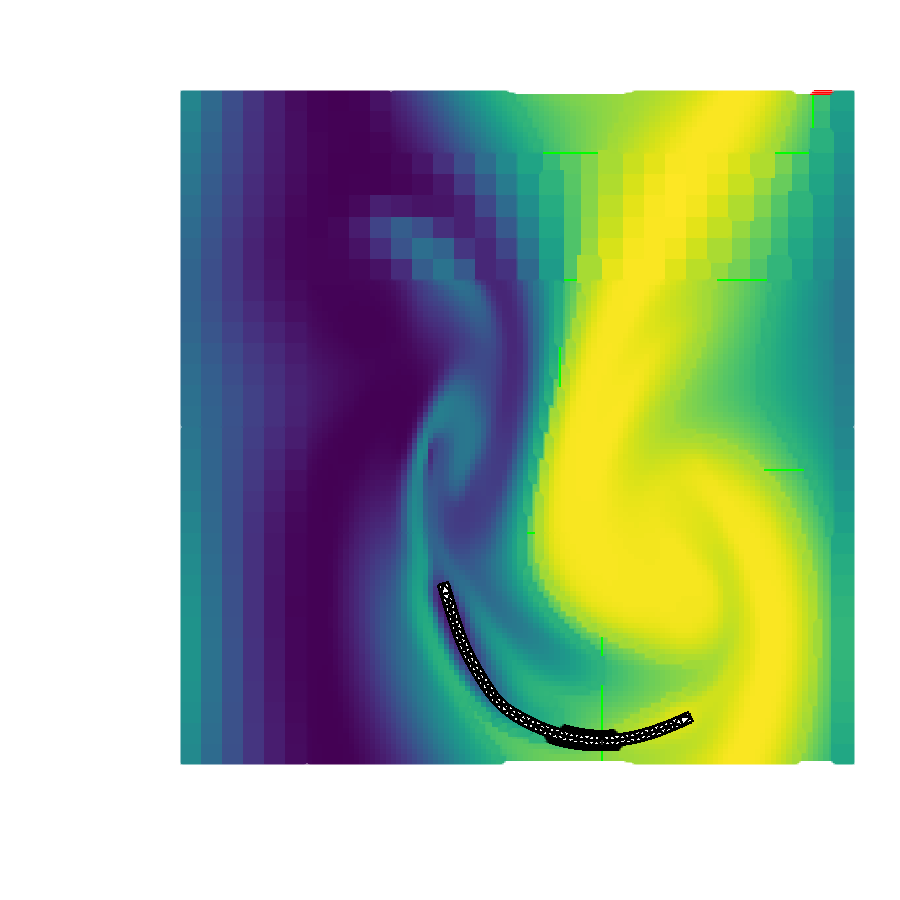
\includegraphics[width=\textwidth]{ch24-predcorr-t4.png}\\ \scriptsize predictor--corrector, $\kappa = 10^{-6}$
\column{0.25\textwidth}\centering 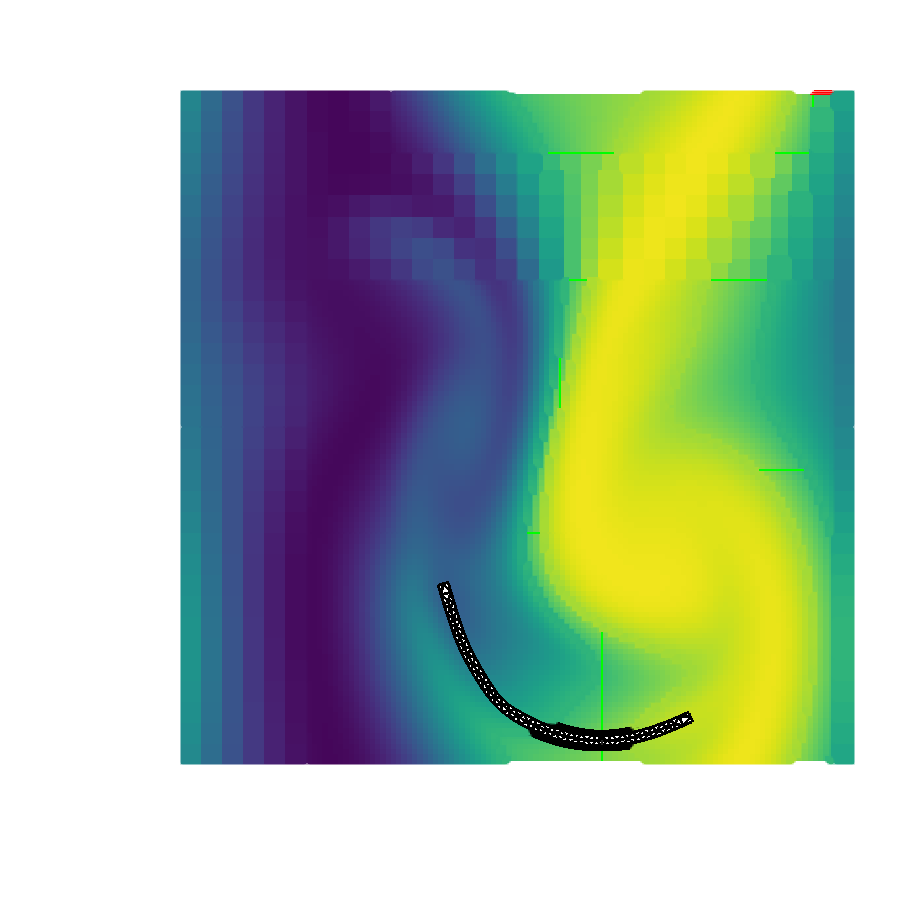
\includegraphics[width=\textwidth]{ch24-kappa1e-3-t4.png}\\ \scriptsize semi-implicit, $\kappa = 10^{-3}$
\column{0.25\textwidth}\centering 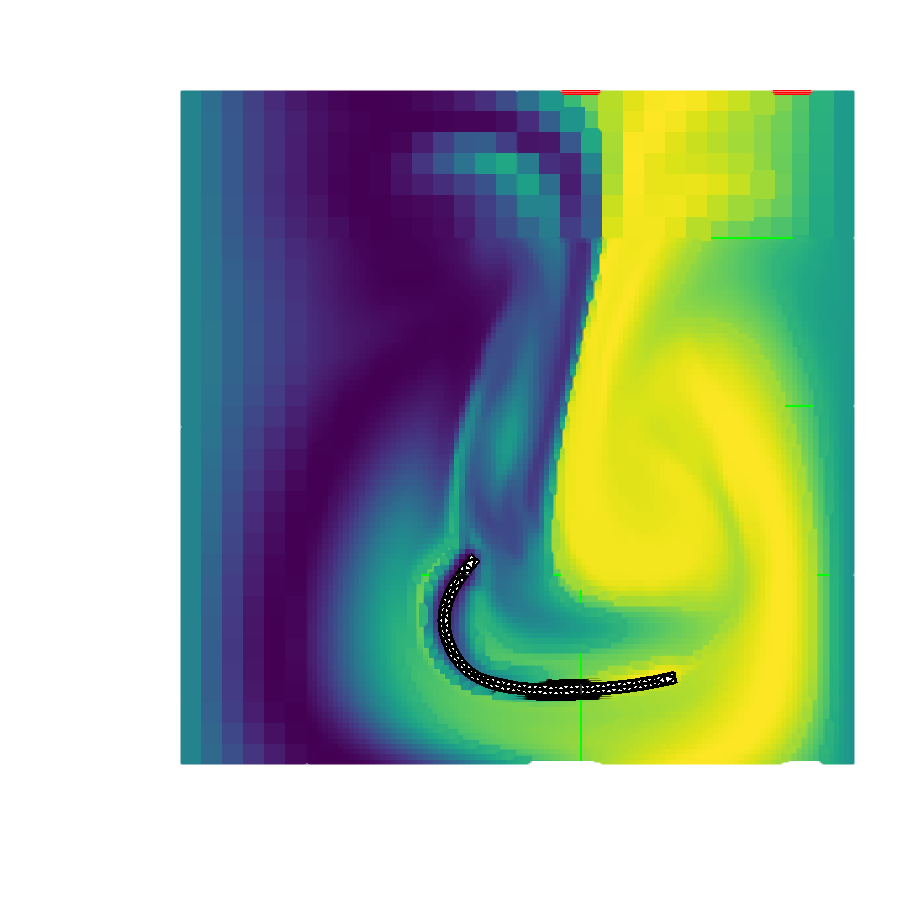
\includegraphics[width=\textwidth]{ch24-walls-t4.png}\\ \scriptsize walls instead of periodic sides
\end{columns}
\footnotesize
\begin{tabular}{@{}L{0.3\textwidth}L{0.62\textwidth}@{}}
\toprule
predictor--corrector & never above the starting maximum ($0.9998$) nor below $-0.0003$; average within $0.4999$--$0.5003$; the largest $T$ falls to $0.9965$ by $t = 4$: no overshoot, slightly worn extremes \\
$\kappa = 10^{-3}$ & diffusion over $\sqrt{\kappa t} = 0.06$, four fine cells, by $t = 4$: the stripes blur; $T$ between $0.017$ and $0.979$; no overshoot; average within $10^{-4}$ of $0.5$ \\
walls & \code{periodic\_dimension = 0,0}: the fluid sticks to the walls and $T$ is held at its initial values there; the plate moves differently (up to $0.15$ at $t = 4$); $T$ between $-0.033$ and $1.015$ \\
\bottomrule
\end{tabular}
\end{frame}

% 13b
\begin{frame}{What you should see (3): the solvers side by side}
\label{fr:solvers2}
\footnotesize
\begin{itemize}
  \item At $\kappa = 10^{-6}$ the two solvers give the same large-scale picture (the stripes, the fold round the plate) and differ in the small things: the semi-implicit scheme overshoots by $0.5\%$ at the folds ($1.008$ at worst over all frames) and undershoots by $0.3\%$; the predictor--corrector's limiter forbids both, and pays with extremes that decay by $0.35\%$ in four time units. Neither is ``right'': the exact solution at this P\'eclet number has stripes thinner than a cell, which no scheme on this grid can hold.
  \item $\kappa = 10^{-3}$ is the honest case for this grid: the physical diffusion ($4$ cells) exceeds the numerical one, both solvers agree closely, and the result converges under refinement (chapter 16's test).
  \item For a quantity that must stay bounded (a concentration, a volume fraction, a probability), use the predictor--corrector, or clip in the post-processing and say so.
  \item The run costs the same either way: $91$ s against IBFE/01's $70$ s on four cores with 0.19.0; the scalar solve is cheap next to the fluid's.
\end{itemize}
\end{frame}

% 14
\begin{frame}{The 2020 deck's last slide: rescaling the tether and the modulus}
\label{fr:rescale}
\scriptsize
\begin{columns}[T]
\column{0.5\textwidth}
``Rescaling kappa\_spring and the elastic modulus. $F = kx$.
\[ k_{\mathrm{new}} = \bigl(k_{\mathrm{old}}\,(F_{\mathrm{new}}/F_{\mathrm{old}})\bigr)\,(ds_{\mathrm{old}}/ds_{\mathrm{new}}), \qquad F \sim \rho L U^2. \]
Elastic modulus: try leaving it the same. Scale mu and beta with e'' (2020, slide 18), followed by the \code{E\_STEM}, \code{E\_LEAF}, \code{MU\_*}, \code{BETA\_*} lines of chapter 22 with $E = 10^7$.
\begin{itemize}
  \item The slide answers a question from the room, not the chapter: ``I changed the units (or the grid) and the plate went limp (or exploded): how do I move the stiffnesses?''
  \item \al{The tether.} The tether force per point is $\kappa_s\,\Delta x$, and the force it must balance scales with the fluid's $\rho L U^2$ (chapter 8b). Change the problem's scale and $\kappa_s$ scales with $F_{\mathrm{new}}/F_{\mathrm{old}}$; change the mesh spacing and the force per point must change with the number of points per length, $ds_{\mathrm{old}}/ds_{\mathrm{new}}$. Both factors are on the slide.
\end{itemize}
\column{0.48\textwidth}
\begin{itemize}
  \item \al{The modulus.} $E$ (and $\mu_s$, $\beta$ with it) is a stress, force per area: it does not change with the mesh at all, and with the scale it changes like $\rho U^2$. ``Try leaving it the same'' is right when the units are unchanged and only the grid is; otherwise scale it with the dynamic pressure, as chapter 19 (slide 17) did for $\mu_s$.
  \item A cleaner route is chapter 8b's: write the input in terms of the dimensionless groups (the Reynolds number, $\kappa_s/(\rho U^2 L)$, $E/(\rho U^2)$, $\kappa/(UL)$ for the scalar) and let the file compute the constants, so that changing $U$, $L$ or $\mathrm{DX}$ changes nothing you have to think about. IBFE/10's \code{KAPPA\_S = 2.5e1*DX/(DT\^{}2)} is the grid part of that rule written out.
  \item For the scalar itself there is nothing to rescale: $\kappa$ is a physical constant, and its dimensionless form is $1/\mathrm{Pe}$.
\end{itemize}
\end{columns}
\end{frame}

% 15
\begin{frame}{Relatives: the point method, and the course's 2014 archive}
\label{fr:relatives}
\footnotesize
\begin{itemize}
  \item \al{Upstream \code{IB/explicit/ex7}} does the same five calls for a point-method body: a dye \code{Q} with diffusion coefficient \code{D}, transported by the flow round an \code{IBMethod} structure. The scalar machinery does not care which IB method moves the body; chapter 15 ran it.
  \item \al{The course's 2014 point-method examples} (the \code{Advection-Diffusion-Examples-3803} folder of the archive): a peristaltic tube carrying a concentration, and a pulsing body that mixes one. Both are 2014 code for the 3803 build, not checked or ported in this series; their advection--diffusion lines are the same as here, with \code{IBMethod} in place of \code{IBFEMethod}. The tube is IB/22 in the example list, a candidate for a later port; the pulsing body is a research model and stays out.
  \item \al{\code{examples/adv\_diff/}} in IBAMR: the scalar solvers alone, in a prescribed velocity field, with exact solutions: the place to check a scheme, a limiter or a boundary condition before it meets a body.
  \item \al{Two-way coupling} (a scalar that drives the flow: temperature through buoyancy, a concentration through a body force) is the same five calls plus a forcing function that reads \code{T}; IBAMR's \code{examples/navier\_stokes} and the multiphase examples do it. Not covered here.
\end{itemize}
\end{frame}

% 16
\begin{frame}[fragile]{Measuring the scalar, and looking at it}
\label{fr:visit}
\footnotesize
\begin{columns}[T]
\column{0.5\textwidth}
In VisIt (the README's recipe):
\begin{enumerate}
  \item Open \code{viz\_IB2d/dumps.visit}; \textbf{Add $\to$ Pseudocolor $\to$ T}; \textbf{Draw}. \code{T} is there by its program name, next to \code{U}, \code{P}, \code{Omega}, \code{Div U} and \code{F}.
  \item Open \code{viz\_IB2d/output.ex2}; \textbf{Add $\to$ Mesh}; the expression \code{dX = \{dX\_0, dX\_1\}}; \textbf{Operators $\to$ Transforms $\to$ Displace} with \code{dX}.
  \item Fix the colour range to $0$--$1$ (\textbf{Pseudocolor $\to$ Min/Max}), or the overshoots and the jump of slide \ref{fr:jump} rescale every frame.
\end{enumerate}
The tables of slides \ref{fr:see}--\ref{fr:variants} are VisIt queries (chapter 29): \textbf{Query $\to$ MinMax} on \code{T} for the extremes, \textbf{Weighted Variable Sum} divided by the box's area for the average, and a \textbf{Pick} at $(0.97, 0.03)$ for the course run's cell by the seam.
\column{0.48\textwidth}
\begin{itemize}
  \item \code{output\_data} in IBFE/12 is chapter 23's state dump (the hierarchy's \code{U} and \code{P} to HDF5, the mesh and systems to libMesh files). To dump \code{T} with them, add its variable index to the \code{ComponentSelector}:
\end{itemize}
\begin{lstlisting}[style=cpptiny]
hier_data.setFlag(var_db->mapVariableAndContextToIndex(
    T_var, adv_diff_integrator->getCurrentContext()));
\end{lstlisting}
\begin{itemize}
  \item A measurement in the program (the amount of $T$ inside a region, the flux through a line) is chapter 11's loop over patches with \code{T}'s patch data; chapter 33 does the same from the files in Python.
  \item A scalar on the \emph{body} (a temperature of the plate, a surface concentration) is a different object: a libMesh system on the mesh, chapter 19's \code{system\_data}; IBAMR does not advect those.
\end{itemize}
\end{columns}
\end{frame}

% 17
\begin{frame}{What can go wrong}
\label{fr:wrong}
\scriptsize
\renewcommand{\arraystretch}{0.95}
\begin{tabular}{@{}L{0.38\textwidth}L{0.54\textwidth}@{}}
\toprule
symptom & cause and fix \\
\midrule
``attempting to perform 2 cycles of fixed point iteration \ldots coupled advection-diffusion solver = 1'' at step 1 & the predictor--corrector with an Adams--Bashforth fluid solver: \code{init\_convective\_time\_stepping\_type = "FORWARD\_EULER"} (slide \ref{fr:cycles}) \\
the log says the other solver than the input & the solver line is read from a block the input does not set (\code{Main}, slide \ref{fr:code1b}); IBFE/12 prints its choice \\
$T$ far outside its starting range near the box edge & a profile that is not periodic in a periodic box (slide \ref{fr:jump}); or walls with \code{gcoef} that disagree with the initial condition \\
\code{TemperatureBcCoefs} changed, no effect & the box is periodic in that direction; the block is read only on non-periodic faces \\
small over- and undershoots at folds & the semi-implicit scheme at high P\'eclet number; the predictor--corrector, or a larger $\kappa$, or a finer grid \\
$T$ smears though $\kappa$ is tiny & numerical diffusion: $\sqrt{\kappa t}$ is below a cell; refine, or accept and say so \\
the scalar's \code{dt\_max} or \code{cfl} seems ignored & the fluid's step governs; the scalar's limits only bite when smaller \\
a second scalar overwrites the first & the same variable name twice; each \code{CellVariable} needs its own name \\
``Unsupported ADV\_DIFF\_SOLVER\_TYPE'' & a spelling other than \code{SEMI\_IMPLICIT} or \code{PREDICTOR\_CORRECTOR} \\
the body's own temperature & not this machinery: a libMesh system on the mesh (slide \ref{fr:visit}) \\
\bottomrule
\end{tabular}
\end{frame}

% 18
\begin{frame}{What the older decks had that is now Part X}
\label{fr:legacy}
\footnotesize
\begin{tabular}{@{}L{0.46\textwidth}L{0.46\textwidth}@{}}
\toprule
2017--2020 & now \\
\midrule
\code{main\_db->getStringWithDefault(}\newline\code{"adv\_diff\_solver\_type", "PREDICTOR\_CORRECTOR")} with no such line in \code{Main} & \code{ADV\_DIFF\_SOLVER\_TYPE} read at the top level, default \code{SEMI\_IMPLICIT}, printed at start \\
\code{RobinBcCoefStrategy<NDIM>* T\_bc\_coef = NULL;} never deleted & a \code{std::unique\_ptr}; \code{nullptr} \\
\code{T = 0.5 + x} in a periodic box & \code{0.5 + 0.5*sin(2*PI*X\_0/L)}, and walls with matching \code{gcoef} as the alternative \\
the predictor--corrector without a single-cycle first step & \code{init\_convective\_time\_stepping\_type = "FORWARD\_EULER"} ready in the input \\
\code{IBAMR\_config.h}, \code{libMeshEnums::Order}, \code{MathUtilities<double>::equalEps} & chapter 17's list \\
``Temperature'' for the block names with ``(or concentration)'' in the text & kept: the block names are the course's; the scalar is whatever you say it is \\
the rescaling slide with \code{E\_STEM = 1.0e7} and no context & slide \ref{fr:rescale} \\
\bottomrule
\end{tabular}
\end{frame}

% 19
\begin{frame}{Exercises}
\label{fr:exercises}
\footnotesize
\begin{enumerate}
  \item Run IBFE/12 with the course's \code{function = "0.5+X\_0"} and watch $T$ next to $x = \pm1$ in VisIt with the colour range fixed to $0$--$1$; then with the range free. Pick the cell at $(0.97, 0.03)$ at $t = 0$ and $t = 4$.
  \item Switch to the predictor--corrector (with the extra line), and compare the largest $T$ over the run with the semi-implicit solver's.
  \item Put walls round the box and hold $T = 0$ on the left wall and $T = 1$ on the right ($a = 1$, $b = 0$, \code{gcoef\_function\_0 = "0.0"}, \code{\_1 = "1.0"}, and $\partial T/\partial n = 0$ on the top and bottom): a plate stirring a box heated from one side.
  \item $\kappa = 10^{-2}$: how long until the stripes are gone? Compare with $\sqrt{\kappa t} = L/2$.
  \item Add a second scalar \code{C} with its own $\kappa$ and a blob initial condition $\exp(-((x-0.3)^2 + y^2)/0.01)$, and plot both.
  \item Dump \code{T} in \code{output\_data} (slide \ref{fr:visit}) and compute the average of $T$ from the HDF5 file in Python (chapter 33); check it against the table of slide \ref{fr:see}.
  \item Add the five calls to IBFE/08 (chapter 21) and put a dye between the plate and the disc.
\end{enumerate}
\end{frame}

% 20
\begin{frame}{Rules of thumb}
\label{fr:thumb}
\small
\begin{itemize}
  \item Five calls per scalar, one line to couple it; the body never knows.
  \item Periodic box, periodic profile; walls, a boundary value that equals the initial value on the wall.
  \item $\sqrt{\kappa t}$ against the cell size tells you whether the diffusion you see is physical or the scheme's.
  \item The semi-implicit solver by default; the predictor--corrector, with the single-cycle first step, when the scalar must stay bounded.
  \item The scalar's step is the fluid's step; its own limits only bite when smaller.
  \item Fix the colour range before you judge a scalar picture.
  \item Stiffnesses scale with $\rho L U^2$ and with the points per length; moduli with $\rho U^2$ only.
\end{itemize}
\end{frame}

% 21
\begin{frame}{Summary}
\label{fr:summary}
\footnotesize
\begin{enumerate}
  \item A passive scalar obeys $\partial_t T + \mathbf{u}\cdot\nabla T = \kappa\Delta T$ with the IB method's velocity and does not act back; at $\mathrm{Pe} = 5\times10^5$ the grid's smearing, not $\kappa$, sets what you see.
  \item Adding one to an IBFE program: two headers, a solver object registered with the fluid integrator, and for each scalar a cell variable, its $\kappa$, initial condition, boundary conditions (non-periodic faces only) and advection velocity.
  \item The semi-implicit solver shares the fluid's scheme and overshoots slightly at folds; the predictor--corrector is bounded, wears its extremes, and needs the fluid's first step to be single-cycle.
  \item The course's $T = 0.5 + x$ jumped by $2$ where the periodic box wraps, and its solver line was never read; IBFE/12 uses a periodic profile, reads and prints the solver, and ships the single-cycle line.
  \item The run takes $90$ s; $T$ stays between $0$ and $1$ with average $0.5$; the variants (predictor--corrector, $\kappa = 10^{-3}$, walls) behave as the scales predict.
\end{enumerate}
\begin{homebox}
\footnotesize Chapter 25 tours IBAMR's own IBFE examples, \code{ex0} to \code{ex11}, with the map of chapter 23 in hand.
\end{homebox}
\end{frame}

% 23
\begin{frame}{References and credits}
\label{fr:refs}
\scriptsize
\begin{itemize}
  \item Example IBFE/12 of this series (\code{main.cpp}, \code{input2d}, \code{IBFE\_Mesh2D\_128.mat}, README with the measured tables); the runs \code{ibfe12\_final}, \code{ibfe12\_predcorr\_fe}, \code{ibfe12\_kappa1e-3}, \code{ibfe12\_walls} and the course program's \code{orig\_ad\_run} with IBAMR 0.19.0, and \code{ibfe12\_default} with 0.16.0; \code{wsl/final/visit\_ch24.sh}. Figures: VisIt 3.5.
  \item The course material: \emph{8-IBFE with Advection and Diffusion} (July 2017) and \emph{9-IBFE with Advection and Diffusion} (2020; its snapshots and box diagram), the MATH 769 version (2018), and the example zip \code{Example\_IBFE\_TetherForceHalfPlate2D\_advdiff\_2016-11}.
  \item IBAMR 0.19.0: \code{src/adv\_diff/AdvDiffHierarchyIntegrator.cpp}, \code{AdvDiffSemiImplicitHierarchyIntegrator.cpp}, \code{AdvDiffPredictorCorrectorHierarchyIntegrator.cpp}, \code{src/advect/AdvectorExplicitPredictorPatchOps.cpp} (the input keys); \code{examples/IB/explicit/ex7}; \code{examples/adv\_diff/ex0}--\code{ex8}. \url{https://github.com/IBAMR/IBAMR}
  \item Robin boundary conditions: the 2020 deck's slides 8--9 adapted the standard definition (as on Wikipedia's ``Robin boundary condition''); the one-dimensional sign remark is theirs.
\end{itemize}
\end{frame}

\end{document}
